\documentclass{article}

\usepackage{graphicx}
\usepackage{float}

\newcommand{\projectnaam}{Service-oriented architecture}
\newcommand{\team}{Zhong-Xi Lu, Thomas Van Bogaert}

\title{\textmd{\textbf{Gedistribueerde Systemen}}\\\normalsize\vspace{0.1in}\Large{\projectnaam}}
\author{\team}
\date{}
\begin{document}
\maketitle

%\section{Explanation}
	\begin{figure}[H]
		\centering
		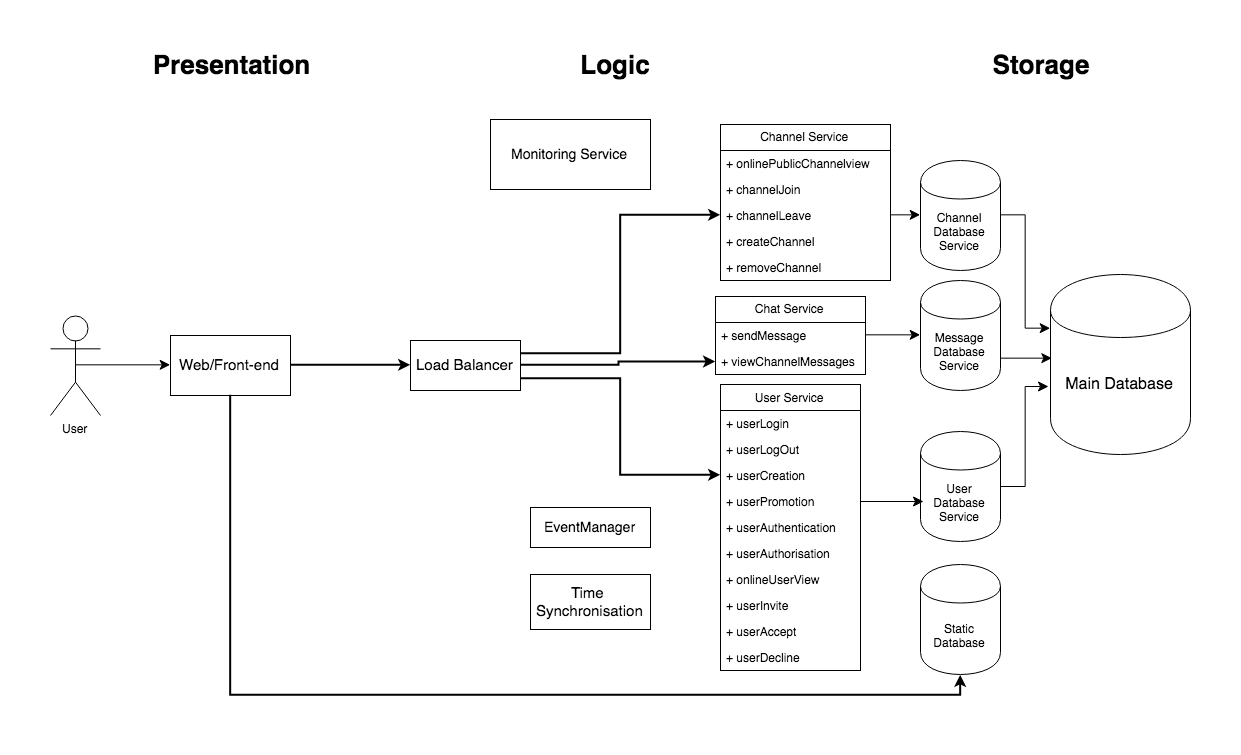
\includegraphics[height=100mm]{architecture.png}
	\end{figure}

	Helemaal links hebben we de User, die de web/frontend kan zien. Daarachter wordt er een request gestuurd die via de Load Balancer naar een server gaat. 
	Op een server is er een Monitoring Service die in controle staat voor alle andere services. De monitoring services zorgen ook voor een overzicht van lopende services. 
	De services kunnen communiceren met elkaar via events. Er is een EventManager om ervoor te zorgen dat services kunnen subscriben aan publishers zonder dat de publisher hier iets van merkt. Hierdoor wordt het mogelijk om asynchrone events over meerdere servers te verdelen.
	Qua storage is er een gemeenschappelijke database voor user-generated data. Deze database zal toegankelijk gemaakt worden door enkele services met elk een vaste API (zie database services). 
	De Static Database dient om alle statische content van de website te voorzien.
	Het is de bedoeling om zo weinig mogelijk staat bij te houden in de individuele services. Dit om te voorkomen dat er veel data tussen de niet-database servers gesynchroniseerd moet worden.


\end{document}